\chapter{Statistics}

\begin{marginfigure}%
  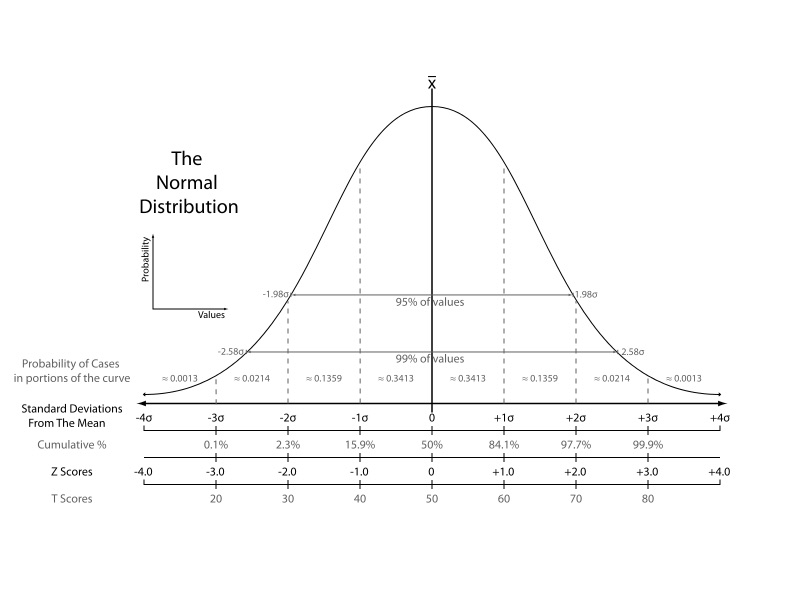
\includegraphics[width=\linewidth]{The_Normal_Distribution}
  \caption{More probability density is found as one gets closer to the expected (mean) value in a normal distribution. Statistics used in standardized testing assessment are shown. The scales include standard deviations, cumulative percentages, percentile equivalents, Z-scores, T-scores, standard nines, and percentages in standard nines..}
  \label{fig:marginfig}
\end{marginfigure}


\normalsize

\section{Introduction}
Statistics is the study of the collection, analysis, interpretation, presentation, and organization of data.[1] In applying statistics to, e.g., a scientific, industrial, or societal problem, it is conventional to begin with a statistical population or a statistical model process to be studied. Populations can be diverse topics such as "all persons living in a country" or "every atom composing a crystal". Statistics deals with all aspects of data including the planning of data collection in terms of the design of surveys and experiments.


%this generates 1cm of vertical space
\vspace{1cm}
\section{Statistics library}

\marginnote[30pt]{In the begin, I need type in "import random" to start this statistics code .}

\marginnote[30pt]{	The first code in statistics library is the explanation of the zero, it is a basic mode to calculate.}

\marginnote[30pt]{The second code is to define the sum of array, it will help user to calculate the sum when the array is longer than affordability.}

\marginnote[30pt]{The third code is to define the rand of array, this code is start more complex than before, we need the n, mini and maxi to finish the calculation}



\begin{shaded}
\begin{verbatim}
import random

def zeros(n):
a=[]
for i in range(n):
a=a+[0]
return a
def sum_array(a):
s=0
for i in range(len(a)):
s=s+a[i]
return s
def rand_array(n,mini,maxi):
a=[]
for i in range(n):
a=a+[random.uniform(mini,maxi)]
return a
def avg(a):
return sum_array(a)/len(a)
def var(a):
s=0
for i in range(len(a)):
s=s+[a[i]**2]
m=avg(a)
return (s/len(a)-m**2)
def maximum(a):
m=-math.inf
for i in range(len(a)):
if a[i]>m:
m=a[i]
return m
\end{verbatim}
\end{shaded}
\marginnote[-200pt]{The fourth code is to know the average of the array, we will use the sum of array devide by lenth of array to calculate this, and we already know how to type the sum of array, so it is not a no clue function. }
\marginnote[-50pt]{In the fifth code, the var is when you define a function parameter and it is a variable number of parameters of meaning, so we can use this code to figure out it very convenient. }

\marginnote[30pt]{The sixth code is to calculate the maximum.}
\marginnote[30pt]{The seventh code is the histogram, we need use the value of mini,maxi,bins and a.}

\marginnote[30pt]{The last two code is bargraph and main, be honest, those two code is relatively strange for me, but in the statistics library, it will be a good supporting code to reduce your time for anytime you need to use those code. }
\begin{shaded}
\begin{verbatim}
def histogram(mini,maxi,bins,a):
h=zeros(bins)
w=(maxi-mini)/bins
for i in range(len(a)):
for j in range(bins):
if a[i]>(mini+j*w) and a[i]<(mini+(j+1)*w):
h[j]=j[j]+1
return h
def bargraph(a):
win=graphWin("BarGraph",400,400)
win.SetCoords(-1,-1,len(a)+1,maximum(a)+1)
for i in range(len(a)):
rec=Rectangle(Point(i,0),Point(i+1,a[i]))
rec.draw(win)
def main():
gauss=[]
for i in range(100):
gauss=gauss+[sum_array(rand_array(10,0,1))]
bargraph(histogram(0,10,10,gauss))

\end{verbatim}
\end{shaded}




